% Filename: lista1.tex
% 
% This code is part of 'Solutions for MS650, M\'{e}todos de Matem\'{a}tica Aplicada II, and F620, M\'{e}todos Matem\'{a}ticos da F\'{i}sica II'
% 
% Description: This file corresponds to the solutions of homework sheet 1.
% 
% Created: 14.07.12 11:13:03 AM
% Last Change: 19.07.12 08:36:46 AM
% 
% Authors:
% - Raniere Silva (2012): initial version
% 
% Copyright (c) 2012 Raniere Silva <r.gaia.cs@gmail.com>
% 
% This work is licensed under the Creative Commons Attribution-ShareAlike 3.0 Unported License. To view a copy of this license, visit http://creativecommons.org/licenses/by-sa/3.0/ or send a letter to Creative Commons, 444 Castro Street, Suite 900, Mountain View, California, 94041, USA.
%
% This work is distributed in the hope that it will be useful, but WITHOUT ANY WARRANTY; without even the implied warranty of MERCHANTABILITY or FITNESS FOR A PARTICULAR PURPOSE.
%
\documentclass[a4paper,12pt, leqno, answers]{exam}
% Customiza\c{c}\~{a}o da classe exam
\newcommand{\mycheader}{Lista 1 - S\'{e}rie de Fourier}
\header{MS560, F560}{\mycheader}{\thepage/\numpages}
\headrule
\footer{Dispon\'{i}vel em \\% Filename: repository.tex
% 
% This code is part of 'Solutions for MS550, M\'{e}todos de Matem\'{a}tica Aplicada I, and F520, M\'{e}todos Matem\'{a}ticos da F\'{i}sica I'
% 
% Description: This file keeps the url of the repository.
% 
% Created: 07.03.12 04:00:00 PM
% Last Change: 14.07.12 10:17:20 AM
% 
% Authors:
% - Raniere Silva (2012): initial version
% 
% Copyright (c) 2012 Raniere Silva <r.gaia.cs@gmail.com>
% 
% This work is licensed under the Creative Commons Attribution-ShareAlike 3.0 Unported License. To view a copy of this license, visit http://creativecommons.org/licenses/by-sa/3.0/ or send a letter to Creative Commons, 444 Castro Street, Suite 900, Mountain View, California, 94041, USA.
%
% This work is distributed in the hope that it will be useful, but WITHOUT ANY WARRANTY; without even the implied warranty of MERCHANTABILITY or FITNESS FOR A PARTICULAR PURPOSE.
%
\url{https://github.com/r-gaia-cs/solucoes_ms650_f620}
}{}{Reportar erros para \\% Filename: maintainer.tex
% 
% This code is part of 'Solutions for MS550, Métodos de Matemática Aplicada I, and F520, Métodos Matemáticos da F\'{i}sica I'
% 
% Description: This file keeps the email of the mainteiner.
% 
% Created: 07.03.12 04:00:00 PM
% Last Change: 30.05.12 04:40:25 PM
% 
% Authors:
% - Raniere Silva (2012): initial version
% 
% Copyright (c) 2012 Raniere Silva <r.gaia.cs@gmail.com>
% 
% This work is licensed under the Creative Commons Attribution-ShareAlike 3.0 Unported License. To view a copy of this license, visit http://creativecommons.org/licenses/by-sa/3.0/ or send a letter to Creative Commons, 444 Castro Street, Suite 900, Mountain View, California, 94041, USA.
%
% This work is distributed in the hope that it will be useful, but WITHOUT ANY WARRANTY; without even the implied warranty of MERCHANTABILITY or FITNESS FOR A PARTICULAR PURPOSE.
%
\href{mailto:r.gaia.cs@gmail.com}{r.gaia.cs@gmail.com}
}
\footrule 
\pagestyle{headandfoot}
\renewcommand{\solutiontitle}{\noindent\textbf{Solu\c{c}\~{a}o:}\enspace}
\SolutionEmphasis{\slshape}
\unframedsolutions
\pointname{}

% Filename: paper_size.tex
%
% This code is part of 'Solutions for MS650, Métodos de Matemática Aplicada II, and F620, Métodos Matemáticos da F\'{i}sica II'
% 
% Description: This file corresponds to the paper size output.
% 
% Created: 14.07.12 11:13:03 AM
% Last Change: 22.08.12 08:24:31 AM
% 
% Authors:
% - Raniere Silva (2012): initial version
% 
% Copyright (c) 2012 Raniere Silva <r.gaia.cs@gmail.com>
% 
% This work is licensed under the Creative Commons Attribution-ShareAlike 3.0 Unported License. To view a copy of this license, visit http://creativecommons.org/licenses/by-sa/3.0/ or send a letter to Creative Commons, 444 Castro Street, Suite 900, Mountain View, California, 94041, USA.
%
% This work is distributed in the hope that it will be useful, but WITHOUT ANY WARRANTY; without even the implied warranty of MERCHANTABILITY or FITNESS FOR A PARTICULAR PURPOSE.
%
% Para impressão
\usepackage[top=3cm, bottom=3cm, left=2cm, right=2cm]{geometry}

% Para ereaders (Kindle, Nook, Kobo, ...)
% \usepackage[papersize={160mm,200mm},margin=2mm]{geometry}
% \sloppy

% Para tablets (iPad, GalaxyTab, ...)
% \usepackage[papersize={140mm,190mm},margin=2mm]{geometry}
% \sloppy


% Filename: packages.tex
% 
% This code is part of 'Solutions for MS650, M\'{e}todos de Matem\'{a}tica Aplicada II, and F620, M\'{e}todos Matem\'{a}ticos da F\'{i}sica II'
% 
% Description: This file corresponds to the packages used.
% 
% Created: 07.03.12 04:00:00 PM
% Last Change: 14.07.12 11:03:30 AM
% 
% Authors:
% - Raniere Silva (2012): initial version
% 
% Copyright (c) 2012 Raniere Silva <r.gaia.cs@gmail.com>
% 
% This work is licensed under the Creative Commons Attribution-ShareAlike 3.0 Unported License. To view a copy of this license, visit http://creativecommons.org/licenses/by-sa/3.0/ or send a letter to Creative Commons, 444 Castro Street, Suite 900, Mountain View, California, 94041, USA.
%
% This work is distributed in the hope that it will be useful, but WITHOUT ANY WARRANTY; without even the implied warranty of MERCHANTABILITY or FITNESS FOR A PARTICULAR PURPOSE.
%
\usepackage[utf8]{inputenc}
\usepackage[T1]{fontenc}
\usepackage[brazil]{babel}
\usepackage{amsmath}
\usepackage{amsfonts}
\usepackage{amssymb}
\usepackage{hyperref}
\usepackage{graphicx}
\usepackage{tikz}

% Customiza\c{c}\~{a}o do pacote amsmath
\allowdisplaybreaks[4]

% Novos comandos
\newcommand{\devd}[2]{\frac{\mathrm{d} #1}{\mathrm{d} #2}}
\newcommand{\devdt}[2]{\frac{\mathrm{d}^2 #1}{\mathrm{d} #2^2}}
\newcommand{\devdtm}[3]{\frac{\mathrm{d}^2 #1}{\mathrm{d} #2 \mathrm{d} #3}}
\newcommand{\devp}[2]{\frac{\partial #1}{\partial #2}}
\newcommand{\grad}{\mbox{grad }}
\newcommand{\diver}{\mbox{div }}
\newcommand{\rot}{\mbox{rot }}

\newcommand{\id}[1]{\, \mathrm{d}#1}


\begin{document}
%cover
\thispagestyle{empty}
% Filename: cover.tex
% 
% This code is part of 'Solutions for MS650, Métodos de Matemática Aplicada II, and F620, Métodos Matemáticos da F\'{i}sica II'
% 
% Description: This file corresponds to the cover.
% 
% Created: 14.07.12 11:18:08 AM
% Last Change: 14.07.12 11:18:08 AM
% 
% Authors:
% - Raniere Silva (2012): initial version
% 
% Copyright (c) 2012 Raniere Silva <r.gaia.cs@gmail.com>
% 
% This work is licensed under the Creative Commons Attribution-ShareAlike 3.0 Unported License. To view a copy of this license, visit http://creativecommons.org/licenses/by-sa/3.0/ or send a letter to Creative Commons, 444 Castro Street, Suite 900, Mountain View, California, 94041, USA.
%
% This work is distributed in the hope that it will be useful, but WITHOUT ANY WARRANTY; without even the implied warranty of MERCHANTABILITY or FITNESS FOR A PARTICULAR PURPOSE.
%
\begin{center}
    \LARGE{Soluções para MS650, Métodos de Matemática Aplicada II, e F620, Métodos Matemáticos da F\'{i}sica II}
    
    \Large{\mycheader}
\end{center}
\vspace{.5\textheight}

\begin{tabular}{|p{.9\textwidth}|}
\hline
Este trabalho foi licenciado com a Licença Creative Commons Atribuição - CompartilhaIgual 3.0 Não Adaptada. Para ver uma c\'{o}pia desta licença, visite \url{http://creativecommons.org/licenses/by-sa/3.0/} ou envie um pedido por carta para Creative Commons, 444 Castro Street, Suite 900, Mountain View, California, 94041, USA.
\begin{center}

\includegraphics[scale=1]{cc-by-sa.png}
\end{center}
Este trabalho encontra-se dispon\'{i}vel em % Filename: repository.tex
% 
% This code is part of 'Solutions for MS550, M\'{e}todos de Matem\'{a}tica Aplicada I, and F520, M\'{e}todos Matem\'{a}ticos da F\'{i}sica I'
% 
% Description: This file keeps the url of the repository.
% 
% Created: 07.03.12 04:00:00 PM
% Last Change: 14.07.12 10:17:20 AM
% 
% Authors:
% - Raniere Silva (2012): initial version
% 
% Copyright (c) 2012 Raniere Silva <r.gaia.cs@gmail.com>
% 
% This work is licensed under the Creative Commons Attribution-ShareAlike 3.0 Unported License. To view a copy of this license, visit http://creativecommons.org/licenses/by-sa/3.0/ or send a letter to Creative Commons, 444 Castro Street, Suite 900, Mountain View, California, 94041, USA.
%
% This work is distributed in the hope that it will be useful, but WITHOUT ANY WARRANTY; without even the implied warranty of MERCHANTABILITY or FITNESS FOR A PARTICULAR PURPOSE.
%
\url{https://github.com/r-gaia-cs/solucoes_ms650_f620}
 e atualmente é mantido por % Filename: maintainer_name.tex
% 
% This code is part of 'Solutions for MS550, Métodos de Matemática Aplicada I, and F520, Métodos Matemáticos da F\'{i}sica I'
% 
% Description: This file keeps the email of the mainteiner.
% 
% Created: 02.08.12 10:41:35 PM
% Last Change: 02.08.12 10:41:35 PM
% 
% Authors:
% - Raniere Silva (2012): initial version
% 
% Copyright (c) 2012 Raniere Silva <r.gaia.cs@gmail.com>
% 
% This work is licensed under the Creative Commons Attribution-ShareAlike 3.0 Unported License. To view a copy of this license, visit http://creativecommons.org/licenses/by-sa/3.0/ or send a letter to Creative Commons, 444 Castro Street, Suite 900, Mountain View, California, 94041, USA.
%
% This work is distributed in the hope that it will be useful, but WITHOUT ANY WARRANTY; without even the implied warranty of MERCHANTABILITY or FITNESS FOR A PARTICULAR PURPOSE.
%
Raniere Silva
 (% Filename: maintainer.tex
% 
% This code is part of 'Solutions for MS550, Métodos de Matemática Aplicada I, and F520, Métodos Matemáticos da F\'{i}sica I'
% 
% Description: This file keeps the email of the mainteiner.
% 
% Created: 07.03.12 04:00:00 PM
% Last Change: 30.05.12 04:40:25 PM
% 
% Authors:
% - Raniere Silva (2012): initial version
% 
% Copyright (c) 2012 Raniere Silva <r.gaia.cs@gmail.com>
% 
% This work is licensed under the Creative Commons Attribution-ShareAlike 3.0 Unported License. To view a copy of this license, visit http://creativecommons.org/licenses/by-sa/3.0/ or send a letter to Creative Commons, 444 Castro Street, Suite 900, Mountain View, California, 94041, USA.
%
% This work is distributed in the hope that it will be useful, but WITHOUT ANY WARRANTY; without even the implied warranty of MERCHANTABILITY or FITNESS FOR A PARTICULAR PURPOSE.
%
\href{mailto:r.gaia.cs@gmail.com}{r.gaia.cs@gmail.com}
).

Este trabalho é distribuido na esperança que possa ser \'{u}til, mas SEM NENHUMA GARANTIA; sem uma garantia implicita de ADEQUA\c{C}\~{A}O a qualquer MERCADO ou APLICA\c{C}\~{A}O EM PARTICULAR.
\\ \hline
\end{tabular}

\newpage
\setcounter{page}{1}

Algumas express\~{o}es eventualmente \'{u}teis:
\begin{align}
    & f(x) = \frac{a_0}{2} + \sum_{r = 1}^\infty \left[ a_r \cos\left( \frac{2 \pi r x}{L} \right) + b_r \sin\left( \frac{2 \pi r x}{L} \right) \right] \label{eq:serie_fourier} \\
    & a_r = \frac{2}{L} \int_{x_0}^{x_0 + L} f(x) \cos\left( \frac{2 \pi r x}{L} \right) \id{x} \label{eq:serie_fourier_a} \\
    & b_r = \frac{2}{L} \int_{x_0}^{x_0 + L} f(x) \sin\left( \frac{2 \pi r x}{L} \right) \id{x} \label{eq:serie_fourier_b}
\end{align}
\begin{questions}
    \question Escreva a s\'{e}rie de Fourier no intervalor $(-\pi, \pi)$ das seguintes fun\c{c}\~{o}es e esboce os gr\'{a}fico das fun\c{c}\~{o}es representadas por essas s\'{e}ries para todo $x$:
    \begin{parts}
        \part $f(x) = \begin{cases}
            -\pi, & - \pi < x < 0, \\
            x, & 0 < x < \pi.
        \end{cases}$
        \begin{solution}
            Temos que
            \begin{align*}
                a_0 &= \frac{1}{\pi} \int_{-\pi}^\pi f(x) \id{x} \\
                &= \frac{1}{\pi} \int_{-\pi}^0 \left( -\pi \right) \id{x} + \frac{1}{\pi} \int_0^\pi x \id{x} \\
                &= \frac{1}{\pi} \left( -\pi \right) \left. x \right|_{-\pi}^0 + \frac{1}{\pi 2} \left. x^2 \right|_0^\pi \\
                &= -\left( 0 - \left( -\pi \right) \right) + \frac{1}{2 \pi} \left( \pi^2 - 0 \right) \\
                &= -\pi + \frac{\pi}{2} \\
                &= \frac{-\pi}{2} \\
                a_n &= \frac{1}{\pi} \int_{-\pi}^\pi f(x) \cos\left( n x \right) \id{x} \\
                &= \frac{1}{\pi} \left[ \int_{-\pi}^0 \left( -\pi \right) \cos\left( n x \right) \id{x} + \int_0^\pi x \cos\left( n x \right) \id{x} \right] \\
                &= - \int_{-\pi}^0 \cos\left( n x \right) \id{x} + \frac{1}{\pi} \int_0^\pi x \cos\left( n x \right) \id{x} \\
                &= - \left. \frac{\sin\left( n x \right)}{n} \right|_{-\pi}^0 + \frac{1}{\pi} \left[ \left. \frac{x \sin\left( n x \right)}{n} \right|_0^\pi - \int_0^\pi \frac{\sin\left( n x \right)}{n} \id{x} \right] \\
                &= - \left( 0 - \frac{\sin\left( -n \pi \right)}{n} \right) + \frac{1}{\pi} \left[ \pi \frac{\sin\left( n \pi \right)}{n} - 0 + \frac{1}{n} \int_0^\pi \left( - \sin\left( n x \right) \right) \id{x} \right] \\
                &= \frac{1}{n \pi}\left. \frac{\cos\left( n x \right)}{n} \right|_0^\pi \\
                &= \frac{1}{n^2 \pi} \left( \cos\left( n \pi \right) - \cos(0) \right) \\
                &= \frac{1}{n^2 \pi} \left( (-1)^n - 1 \right) \\
                &= \frac{(-1)^n - 1}{n^2 \pi} \\
                b_n &= \frac{1}{\pi} \int_{-\pi}^\pi f(x) \sin\left( n x \right) \id{x} \\
                &= \frac{1}{\pi} \left[ \int_{-\pi}^0 \left( -\pi \right) \sin\left( n x \right) \id{x} + \int_0^\pi x \sin\left( n x \right) \id{x} \right] \\
                &= \int_{-\pi}^0 \left( -\sin\left( n x \right) \right) \id{x} + \frac{1}{\pi} \int_0^\pi x \sin\left( n x \right) \id{x} \\
                &= \left. \frac{\cos\left( n x \right)}{n} \right|_{-\pi}^0 + \frac{1}{\pi} \left[ \left. x \frac{\left( -\cos\left( n x \right) \right)}{n} \right|_0^\pi + \int_0^\pi \frac{\cos\left( n x \right)}{n} \id{x} \right] \\
                &= \frac{1}{n} \left( 1 - \cos\left( - n \pi \right) \right) - \frac{1}{n \pi} \left( \pi \cos\left( n \pi \right) - 0 \right) + \frac{1}{n} \left. \frac{\sin\left( n x \right)}{n} \right|_0^\pi \\
                &= \frac{1 - \left( -1 \right)^n}{n} - \frac{1}{n} (-1)^n + \frac{1}{n^2} \left( \sin\left( n \pi \right) - 0 \right) \\
                &= \frac{1 - (-1)^n - (-1)^n}{n} \\
                &= \frac{1 - 2 (-1)^n}{n}.
            \end{align*}
            Portanto,
            \begin{align*}
                f(x) &= \frac{a_0}{2} + \sum_{n = 1}^\infty \left( a_n \cos\left( n x \right) + b_n \sin\left( n x \right) \right) \\
                &= \frac{-\pi}{4} + \sum_{n = 1}^\infty \left( \frac{(-1)^n - 1}{n^2 \pi} \cos\left( n x \right) + \frac{1 - 2 (-1)^n}{n} \sin\left( n x \right) \right).
            \end{align*}
            % TODO Incluir gr\'{a}fico.
        \end{solution}

        \part $f(x) = | \sin x |, -\pi < x < \pi$.
        \begin{solution}

            Temos que $f(x) = | \sin x |, -\pi < x < \pi$ equivale a
            \begin{align*}
                f(x) &= \begin{cases}
                    \sin x, 0 < x < \pi, \\
                    -\sin x, -\pi < x < \pi,
                \end{cases}
            \end{align*}
            e, portanto,
            \begin{align*}
                a_0 &= \frac{1}{\pi} \int_{-\pi}^\pi f(x) \id{x} \\
                &= \frac{1}{\pi} \left[ \int_{-\pi}^0 \left( - \sin(x) \right) \id{x} + \int_0^\pi \sin(x) \id{x} \right] \\
                &= \frac{1}{\pi} \left[ \left. \cos(x) \right|_{-\pi}^0 + \left. \left( -\cos(x) \right) \right|_0^\pi \right] \\
                &= \frac{1}{\pi} \left[ 1 - (-1) - \left( -1 - 1 \right) \right] \\
                &= \frac{4}{\pi}, \\
                a_n &= \frac{1}{\pi} \int_{-\pi}^\pi f(x) \cos\left( n x \right) \id{x} \\
                &= \frac{1}{\pi} \left[ -\int_{-\pi}^0 \sin\left( x \right) \cos\left( n x \right) \id{x} + \int_0^\pi \sin\left( x \right) \cos\left( n x \right) \id{x} \right] \\
                \begin{split}
                    &= - \frac{1}{\pi} \int_{-\pi}^0 \frac{1}{2} \left( \sin\left( (1 + n) x \right) + \sin\left( (1 - n) x \right) \right) \id{x} \\
                    &\quad {}+ \frac{1}{\pi} \int_0^\pi \frac{1}{2} \left( \sin\left( (1 + n) x \right) + \sin\left( (1 - n) x \right) \right) \id{x} \\
                \end{split} \\
                \begin{split}
                    &= - \frac{1}{2 \pi} \int_{-\pi}^0 \sin\left( (1 + n) x \right) \id{x} - \frac{1}{2 \pi} \int_{-\pi}^0 \sin\left( (1 - n) x \right) \id{x} \\
                    &\quad {}+ \frac{1}{2 \pi} \int_0^\pi \sin\left( (1 + n) x \right) \id{x} + \frac{1}{2 \pi} \int_0^\pi \sin\left( (1 - n) x \right) \id{x}
                \end{split} \\
                \begin{split}
                    &= \frac{1}{2 \pi} \left. \frac{\cos\left( (1 + n) x \right)}{1 + n} \right|_{-\pi}^0 + \frac{1}{2 \pi} \left. \frac{\cos\left( (1 - n) x \right)}{1 - n} \right|_{-\pi}^0 \\
                    &\quad {}- \frac{1}{2 \pi} \left. \frac{\cos\left( (1 + n) x \right)}{1 + n} \right|_0^\pi - \frac{1}{2 \pi} \left. \frac{\cos\left( (1 - n) x \right)}{1 - n} \right|_0^\pi
                \end{split} \\
                % TODO Incluir passagens intermedi\'{a}rias.
                &= \frac{1 - (-1)^{n + 1}}{\pi} \left[ \frac{1}{1 + n} + \frac{1}{1 - n} \right].
            \end{align*} 
            % TODO Escrever solu\c{c}\~{a}o.
        \end{solution}

        \part $f(x) = \begin{cases}
            -x, & -\pi < x < 0, \\
            x, & 0 < x < \pi.
        \end{cases}$
        \begin{solution}
            % TODO Escrever solu\c{c}\~{a}o.
        \end{solution}

        \part $f(x) = \cosh x, -\pi < x < \pi$.
        \begin{solution}
            % TODO Escrever solu\c{c}\~{a}o.
        \end{solution}

        \part $f(x) = \begin{cases}
            0, & -\pi < x < 0, \\
            x, & 0 < x < \pi/2, \\
            \pi - x, & \pi/2 < x < \pi.
        \end{cases}$
        \begin{solution}
            % TODO Escrever solu\c{c}\~{a}o.
        \end{solution}
    \end{parts}

    \question Escreva a fun\c{c}\~{a}o $f(x) = x^2 / 4$ em s\'{e}rie de Fourier no intervalo $(-\pi, \pi)$ e use o resultado para mostrar que 
    \begin{align*}
        1 + \frac{1}{4} + \frac{1}{9} + \frac{1}{16} + \ldots &= \frac{\pi^2}{6}, \\
        1 - \frac{1}{4} + \frac{1}{9} - \frac{1}{16} + \ldots &= \frac{\pi^2}{12}, \\
        1 + \frac{1}{9} + \frac{1}{25} + \frac{1}{49} + \ldots &= \frac{\pi^2}{8}.
    \end{align*}
    \begin{solution}
        % TODO Escrever solu\c{c}\~{a}o.
    \end{solution}

    \question Escreva as s\'{e}ries de Fourier sobre o intervalo $(-\pi, \pi)$ para as fun\c{c}\~{o}es abaixo:
    \begin{parts}
        \part $f(x) = \begin{cases}
            0, & -\pi < x < 0, \\
            \sin x, & 0 < x < \pi.
        \end{cases}$
        \begin{solution}
            % TODO Escrever solu\c{c}\~{a}o.
        \end{solution}

        \part $f(x) = \exp(x)$.
        \begin{solution}
            % TODO Escrever solu\c{c}\~{a}o.
        \end{solution}
    \end{parts}

    \question Use a representa\c{c}\~{a}o na forma complexa da s\'{e}rie de Fourier para escrever a s\'{e}rie correspondente \`{a} fun\c{c}\~{a}o $f(x) = \exp x$, $-\pi < x < \pi$ e compare esse resultado com o exerc\'{i}cio anterior.
    \begin{solution}
        % TODO Escrever solu\c{c}\~{a}o.
    \end{solution}

    \question Escreva a fun\c{c}ao $f(x) = \left( \pi - x \right) / 2$ em uma s\'{e}rie de Fourier no intervalo $(-\pi, \pi)$ e use o resultado para mostrar que 
    \begin{align*}
        \sum_{n = 1}^\infty \frac{1}{n^2} &= \frac{\pi^2}{6}.
    \end{align*}
    \begin{solution}
        % TODO Escrever solu\c{c}\~{a}o.
    \end{solution}

    \question Escreva a s\'{e}rie de cossenos e a s\'{e}rie de senos de Fourier correspondente \`{a}s fun\c{c}\~{o}es abaixo e esboce o gr\'{a}fico da fun\c{c}\~{a}o representada por essas s\'{e}ries para todo $x$.
    \begin{parts}
        \part $f(x) = 1, 0 < x < \pi$.
        \begin{solution}
            % TODO Escrever solu\c{c}\~{a}o.
        \end{solution}

        \part $f(x) = \pi - x, 0 < x < \pi$.
        \begin{solution}
            % TODO Escrever solu\c{c}\~{a}o.
        \end{solution}

        \part $f(x) = \begin{cases}
            1, & 0 < x < \pi/2, \\
            0, & \pi/2 < x < \pi.
        \end{cases}$
        \begin{solution}
            % TODO Escrver solu\c{c}\~{a}o.
        \end{solution}
    \end{parts}

    \question Escreva a s\'{e}rie de Fourier sobre o intervalo $(0, 2\pi)$ para a fun\c{c}\~{a}o $f(x) = x^2$ e esboce o gr\'{a}fico da fun\c{c}\~{a}o representada por essa s\'{e}rie para todo $x$.
    \begin{solution}
        % TODO Escrver solu\c{c}\~{a}o.
    \end{solution}

    \question Escreva a s\'{e}rie em senos de Fourier sobre o intervalo $(0, 1)$ para a fun\c{c}\~{a}o $f(x) = \cos(\pi x)$.
    \begin{solution}
        % TODO Escrver solu\c{c}\~{a}o.
    \end{solution}

    \question[P1 de 2006] Considdere a fun\c{c}\~{a}o $f(x) = x^3 + 1$.
    % TODO Escrever integra\c{c}\~{a}o.
    \begin{parts}
        \part Encontre sua s\'{e}rie de Fourier no intervalo $(-\pi,\pi)$;
        \begin{solution}
            Temos que
            \begin{align*}
                a_0 &= \frac{1}{\pi} \int_{-\pi}^\pi \left( x^3 + 1 \right) \id{x} \\
                &= \frac{1}{4} \left. \left( \frac{x^4}{4} + x \right) \right|_{-\pi}^\pi \\
                &= 2 \pi / \pi = 2, \\
                a_n &= \frac{1}{\pi} \int_{-\pi}^\pi \left( x^3 + 1 \right) \cos\left( n x \right) \id{x} \\
                \begin{split}
                    &= \frac{1}{\pi} \left. \frac{\sin\left( n x \right)}{n} \right|_{-\pi}^\pi + \frac{1}{\pi} \frac{3 \pi^2 \cos\left( n \pi \right)}{n^2} - \frac{1}{\pi} \frac{3 (-\pi)^2 \cos\left( -n \pi \right)}{n^2} \\
                    &\quad {}- \frac{1}{\pi} \frac{6}{n^4} \cos\left( n \pi \right) + \frac{6}{n^4} \cos\left( -n \pi \right)
                \end{split} \\
                &= 0, \\
                b_n &= \frac{1}{\pi} \int_{-\pi}^\pi \left( x^3 + 1 \right) \sin\left( n x \right) \id{x} \\
                \begin{split}
                    &= \frac{1}{\pi} \left. \frac{- \cos\left( n x \right)}{n} \right|_{-\pi}^\pi - \frac{1}{\pi} \frac{\pi^3 \cos\left( n \pi \right)}{n} - \frac{1}{\pi} \frac{- (-\pi)^3 \cos\left( - n \pi \right)}{n} \\
                    &\quad {}+ \frac{1}{\pi} \frac{6 \pi \cos\left( n \pi \right)}{n^3} - \frac{1}{\pi} \frac{6 (-\pi) \cos\left( n (-\pi) \right)}{n^3}
                \end{split} \\
                &= \frac{2 (-1)^n [6 - \pi^2 n^2]}{n^3}.
            \end{align*}
            Portanto,
            \begin{align*}
                F[f](x) &= 1 + \sum_{n = 1}^\infty \frac{2 (-1)^n (6 - \pi^2 n^2)}{n^3} \sin\left( n x \right).
            \end{align*}
        \end{solution}

        \part Encontre sua s\'{e}rie de Fourier em senos no intervalo $(0,\pi)$;
        \begin{solution}
            Temos que
            \begin{align*}
                b_n &= \frac{2}{\pi} \int_0^\pi \left( x^3 + 1 \right) \sin\left( n x \right) \id{x} \\
                &= \frac{2}{\pi} \left[ \left. \frac{-\cos\left( n x \right)}{n} \right|_0^\pi - \frac{\pi^3 \cos\left( n \pi \right)}{n} + \frac{6 \pi \cos\left( n \pi \right)}{n^3} \right] \\
                &= \frac{2 (-1)^n}{\pi n} \left[ -1 + (-1)^n - \pi^3 + \frac{6 \pi}{n^2} \right].
            \end{align*}
            Portanto,
            \begin{align*}
                F_s[f](x) &= \sum_{n = 1}^\infty \frac{2 (-1)^n}{\pi n} \left[ (-1)^n - 1 - \frac{\pi}{n^2} \left( 6 + \pi^2 n^2 \right) \right] \sin\left( n x \right).
            \end{align*}
        \end{solution}

        \part Enconre sua s\'{e}rie de Fourier em cossenos no intervalo $(-\pi,0)$;
        \begin{solution}
            Temos que
            \begin{align*}
                a_0 &= \frac{2}{\pi} \int_{-\pi}^0 \left( x^3 + 1 \right) \id{x} \\
                &= \frac{2}{\pi} \left. \left( \frac{x^4}{4} + x \right) \right|_{-\pi}^0 \\
                &= 2 \left( 1 - \frac{\pi^3}{4} \right), \\
                a_n &= \frac{2}{\pi} \int_{-\pi}^0 \left( x^3 + 1 \right) \cos\left( n x \right) \id{x} \\
                &= \frac{2}{\pi} \left[ \left. \frac{\sin\left( n x \right)}{n} \right|_{-\pi}^0 - \frac{3 \pi^2 \cos\left( n \pi \right)}{n^2} - \frac{6}{n^4} + \frac{6 (-1)^n}{n^4} \right] \\
                &= \frac{12}{\pi n^4} \left[ (-1)^n \left( 1 - \frac{\pi^2 n^2}{2} \right) - 1 \right].
            \end{align*}
            Portanto,
            \begin{align*}
                F_c[f](x) &= \left( 1 - \frac{\pi^3}{4} \right) + \sum_{n = 1}^\infty \frac{12}{\pi n^4} \left[ (-1)^n \left( 1 - \frac{\pi^2 n^2}{2} \right) - 1 \right] \cos\left( n x \right).
            \end{align*}
        \end{solution}

        \part Fa\c{c}a um esbo\c{c}o do gr\'{a}fico das fun\c{c}\~{o}es representadas pelas s\'{e}ries obtidas nos itens anteriores para todo $x \in \mathbb{R}$.
        \begin{solution}
            % TODO Escrever solu\c{c}\~{a}o.
        \end{solution}
    \end{parts}

    \question[P1 de 2006] Seja $f(x)$ uma fun\c{c}\~{a}o satisfazendo a propriedade
    \begin{align*}
        f(x + L) &= -f(x), && L > 0,
    \end{align*}
    para todo $x \in \mathbb{R}$. Mostre que todos os coeficientes pares da sua s\'{e}rie de Fourier no intervalor $(a, a + 2 L)$ s\~{a}o nulos, ou seja,
    \begin{align*}
        & a_0 = a_2 = a_4 = \ldots = 0, \\
        & b_2 = b_4 = b_6 = \ldots = 0.
    \end{align*}
    \begin{solution}
        % TODO Escrever solu\c{c}\~{a}o.
        Do formul\'{a}rio temos que $\alpha = a$ e $\beta = a + 2 l$, portanto
        \begin{align*}
            a_0 &= \frac{1}{L} \int_a^{a + 2 L} f(x) \id{x} \\
            &= \frac{1}{L} \int_a^{a + L} f(x) \id{x} + \frac{1}{L} \int_{a + L}^{a + 2 L} f(x) \id{x} \\
            &= \frac{1}{L} \int_a^{a + L} f(x) \id{x} + \frac{1}{L} \int_a^{a + L} f(\xi + L) \id{\xi} \\
            &= 0, \\
            a_n &= \frac{1}{L} \int_a^{a + 2 L} f(x) \cos\left( \frac{n \pi x}{L} \right) \id{x} \\
            &= \frac{1}{L} \int_a^{a + L} f(x) \cos\left( \frac{n \pi x}{L} \right) \id{x} + \frac{1}{L} \int_{a + L}^{a + 2 L} f(x) \cos\left( \frac{n \pi x}{L} \right) \id{x} \\
            &= \frac{1}{L} \int_a^{a + L} f(x) \cos\left( \frac{n \pi x}{L} \right) \id{x} + \frac{1}{L} \int_a^{a + L} f(\xi + L) \cos\left( \frac{n \pi \xi}{L} + n \pi \right) \id{\xi} \\
            &= \frac{1}{L} \int_a^{a + L} f(x) \cos\left( \frac{n \pi x}{L} \right) \id{x} - (-1)^n \frac{1}{L} \int_a^{a + L} f(\xi) \cos\left( \frac{n \pi \xi}{L} \right) \id{\xi} \\
            &= \begin{cases}
                0, & n \text{ \'{e} par}, \\
                2(\ldots), & n \text{ \'{e} \'{i}mpar},
            \end{cases} \\
            b_n &= \frac{1}{L} \int_a^{a + 2 L} f(x) \sin\left( \frac{n \pi x}{L} \right) \id{x} \\
            &= \frac{1}{L} \int_a^{a + L} f(x) \sin\left( \frac{n \pi x}{L} \right) \id{x} + \frac{1}{L} \int_{a + L}^{a + 2 L} f(x) \sin\left( \frac{n \pi x}{L} \right) \id{x} \\
            &= \frac{1}{L} \int_a^{a + L} f(x) \sin\left( \frac{n \pi x}{L} \right) \id{x} + \frac{1}{L} \int_a^{a + L} f(\xi + L) \sin\left( \frac{n \pi \xi}{L} + n \pi \right) \id{\xi} \\
            &= \frac{1}{L} \int_a^{a + L} f(x) \sin\left( \frac{n \pi x}{L} \right) \id{x} - (-1)^n \frac{1}{L} \int_a^{a + L} f(\xi) \sin\left( \frac{n \pi \xi}{L} \right) \id{\xi} \\
            &= \begin{cases}
                0, & n \text{ \'{e} par}, \\
                2 (\ldots), & n \text{ \'{e} \'{i}mpar}.
            \end{cases}
        \end{align*}
    \end{solution}

    \question[T2 de 2008] Calcule $\int_{-\infty}^\infty \sin\left( x \right) / x \id{x}$.
    \begin{solution}
        Considere o caminho no plano complexo representado na figura abaixo.
        \begin{center}
            \begin{tikzpicture}
                \draw[->] (-4.2,0) -- (4.2,0);
                \draw[->] (0,-.2) -- (0,4.2);
                \draw[line width=2, ->] (4,0) arc (0:60:4) node[above]{$C_R$};
                \draw[line width=2, ->] (60:4) arc (60:120:4);
                \draw[line width=2, ->] (120:4) arc (120:180:4);
                \draw[line width=2, ->] (-4,0) node[below]{$-R$} -- (-1,0) node[below]{$-r$};
                \draw[line width=2, ->] (-1,0) arc (180:120:1);
                \draw[line width=2, ->] (120:1) arc (120:60:1) node[above]{$C_r$};
                \draw[line width=2, ->] (60:1) arc (60:0:1);
                \draw[line width=2, ->] (1,0) node[below]{$r$} -- (4,0) node[below]{$R$};
                \node[below left] at (30:4) {$\Gamma$};
            \end{tikzpicture}
        \end{center}

        Do Teorema de Cauchy, temos que
        \begin{align*}
            \int_\Gamma \frac{\exp\left( i z \right)}{x} \id{z} &= \int_{-R}^{-r} \frac{\exp\left( i z \right)}{z} \id{z} + \int_{C_r} \frac{\exp\left( i z \right)}{z} \id{z} + \int_r^R \frac{\exp\left( i z \right)}{z} \id{z} + \int_{C_R} \frac{\exp\left( i z \right)}{z} = 0.
        \end{align*}
        Por\'{e}m, note que
        \begin{align*}
            \int_{-R}^{-r} \frac{\exp\left( i z \right)}{z} \id{z} + \int)_r^R \frac{\exp\left( i z \right)}{z} \id{z} &= i \int_{-R}^{-r} \frac{\sin\left( z \right)}{z} \id{z} + i \int_r^R \frac{\sin\left( z \right)}{z} \id{z}.
        \end{align*}
        Como $\sin\left( x \right) / x$ \'{e} cont\'{i}nuo em $x = 0$, tem-se
        \begin{align*}
            i \int_{-\infty}^\infty \frac{\sin\left( x \right)}{x} \id{x} = - \lim_{r \to 0} \int_{C_r} \frac{\exp\left( i z \right)}{z} \id{z} - \lim_{R \to \infty} \int_{C_R} \frac{\exp\left( i z \right)}{z} \id{z}.
        \end{align*}
        Fazendo-se uma integra\c{c}\~{a}o por partes
        \begin{align*}
            \int_{C_R} \frac{\exp\left( i z \right)}{z} \id{z} &= \left. \frac{\exp\left( i z \right)}{i z} \right|_R^{-R} - \int_{C_R} \frac{\exp\left( i z \right)}{z^2} \id{z} \\
            &= - \frac{\cos\left( R \right)}{i R} + i \int_0^\pi \frac{\exp\left( i R \exp\left( i \theta \right) \right)}{R \exp\left( 2 i \theta \right)} \id{\theta} \\
            &= 0,
        \end{align*}
        para $R \to \infty$. Para o trecho $C_r$
        \begin{align*}
            \int_{C_r} \frac{\exp\left( i z \right)}{z} \id{z} &= - i \int_0^\pi \exp\left( i r \exp\left( i \theta \right) \right) \id{\theta} \\
            &= - i \pi,
        \end{align*}
        para $r = 0$, de onde finalmente tem-se
        \begin{align*}
            \int_{-\infty}^\infty \frac{\sin\left( x \right)}{x} \id{x} = \pi.
        \end{align*}
    \end{solution}

    \question[T1 de 2011] Encontre a s\'{e}rie em cossenos de Fourier sobre o intervalo $(0, \pi)$ para a fun\c{c}\~{a}o $f(x) = \sin\left( \kappa x \right)$, onde $\kappa$ \'{e} um n\'{u}mero inteiro positivo.
    \begin{solution}
        Temos para $f(x) = \sin\left( \kappa x \right)$, $\kappa = 1, 2, 3 \ldots$ que
        \begin{align*}
            a_0 &= 2 \frac{1}{\pi} \int_0^\pi \sin\left( \kappa x \right) \id{x} \\
            &= \frac{2}{\pi} \left. \left[ \frac{-\cos\left( \kappa x \right)}{\kappa} \right] \right|_0^\pi \\
            &= \frac{2}{\pi \kappa} \left[ 1 - (-1)^\kappa \right] \\
            &= \begin{cases}
                0, & \kappa \text{ \'{e} par}, \\
                4 / \left( \pi \kappa \right), & \kappa \text{ \'{e} \'{i}mpar},
            \end{cases} \\
            a_n &= 2 \frac{1}{\pi} \int_0^\pi \sin\left( \kappa x \right) \cos\left( n x \right) \id{x}, \\
            \intertext{para $n = \kappa$}
            a_k &= \frac{2}{\pi} \int_0^\pi \sin\left( \kappa x \right) \cos\left( \kappa x \right) \id{x} \\
            &= \frac{2}{\pi \kappa} \left. \frac{\sin^2\left( \kappa x \right)}{2} \right|_0^\pi \\
            &= 0, \\
            \intertext{e para $n \neq \kappa$}
            a_n &= \frac{2}{n} \int_0^\pi \frac{1}{2} \left[ \sin\left( \kappa x + n x \right) + \sin\left( \kappa x - n x \right) \right] \id{x} \\
            &= \frac{1}{\pi} \left. \left[ \frac{- \cos\left( (\kappa + n) x \right)}{\kappa + n} - \frac{\cos\left( (k - n) x \right)}{\kappa - n} \right] \right|_0^\pi \\
            &= \frac{1}{\pi} \left[ \frac{1 - (-1)^{n + \kappa}}{\kappa + n} + \frac{1 - (-1)^{n - \kappa}}{\kappa + n} \right] \\
            &= \frac{\left[ 1 - (-1)^{n + \kappa} \right]}{\pi} \frac{2 k}{k^2 - n^2} \\
            &= \begin{cases}
                \frac{\left[ 1 - (-1)^n \right]}{\pi} \frac{2 \kappa}{\kappa^2 - n^2}, & \kappa \text{ \'{e} par}, \\
                \frac{\left[ 1 + (-1)^n \right]}{\pi} \frac{2 \kappa}{\kappa^2 - n^2}, & \kappa \text{ \'{e} \'{i}mpar}.
            \end{cases}
        \end{align*}

        Logo,
        \begin{align*}
            f(x) &= \sum_{m = 0}^\infty \frac{4 \kappa}{\pi} \frac{\cos\left( (2m + 1) x \right)}{\left[ \kappa^2 - (2m + 1)^2 \right]},
        \end{align*}
        quando $k$ \'{e} par e
        \begin{align*}
            f(x) &= \frac{2}{\pi \kappa} + \sum_{m = 1}^\infty \frac{4 \kappa}{\pi} \frac{\cos\left( 2 m x \right)}{\left[ \kappa^2 - 4 m^2 \right]},
        \end{align*}
        quando $\kappa$ \'{e} \'{i}mpar.
    \end{solution}

    \question[P1 de 2011]
    \begin{parts}
        \part Mostre que a s\'{e}rie de Fourier de $\exp(x)$ no intervalo $-\pi < x < \pi$ \'{e} dada por
        \begin{align*}
            S(x) &= \frac{2 \sinh\left( \pi \right)}{\pi} \left[ \frac{1}{2} + \sum_{n = 1}^\infty \frac{(-1)^n}{n^2 + 1} \left( \cos\left( n x \right) - n \sin\left( n x \right) \right) \right].
        \end{align*}
        \begin{solution}
            Temos que
            \begin{align*}
                a_0 &= \frac{1}{\pi} \int_{-\pi}^\pi \exp(x) \id{x} \\
                &= \frac{1}{\pi} \left. \exp(x) \right|_{-\pi}^\pi \\
                &= \frac{2 \sinh\left( \pi \right)}{\pi} \\
                a_n &= \frac{1}{\pi} \int_{-\pi}^\pi \exp(x) \cos\left( n x \right) \id{x} \\
                &= \frac{1}{\pi} \left. \left( \frac{\exp(x) \cos\left( n x \right) + n \exp(x) \sin\left( n x \right)}{1 + n^2} \right) \right|_{-\pi}^\pi \\
                &= \frac{2 \sinh(\pi)}{\pi} \frac{(-1)^n}{1 + n^2}, \\
                b_n &= \frac{1}{\pi} \int_{-\pi}^\pi \exp(x) \sin\left( n x \right) \id{x} \\
                &= \frac{1}{\pi} \left. \left( \frac{\exp(x) \sin\left( n x \right) - n \exp(x) \cos\left( n x \right)}{1 + n^2} \right) \right|_{-\pi}^{\pi} \\
                &= \frac{-2 \sinh(\pi)}{\pi} \frac{(-1)^n}{1 + n^2} n.
            \end{align*}
            Portanto,
            \begin{align*}
                S(x) &= \frac{2 \sinh(\pi)}{\pi} \left[ \frac{1}{2} + \sum_{n = 1}^\infty \frac{(-1)^n}{1 + n^2} \left( \cos\left( n x \right) - n \sin\left( n x \right) \right) \right].
            \end{align*}
        \end{solution}

        \part Fa\c{c}a um esbo\c{c}o do gr\'{a}fico da fun\c{c}\~{a}o representada por essa s\'{e}rie para todo $x \in \mathbb{R}$.
        \begin{solution}
            O esbo\c{c}o encontra-se representado na figura abaixo:
            \begin{center}
                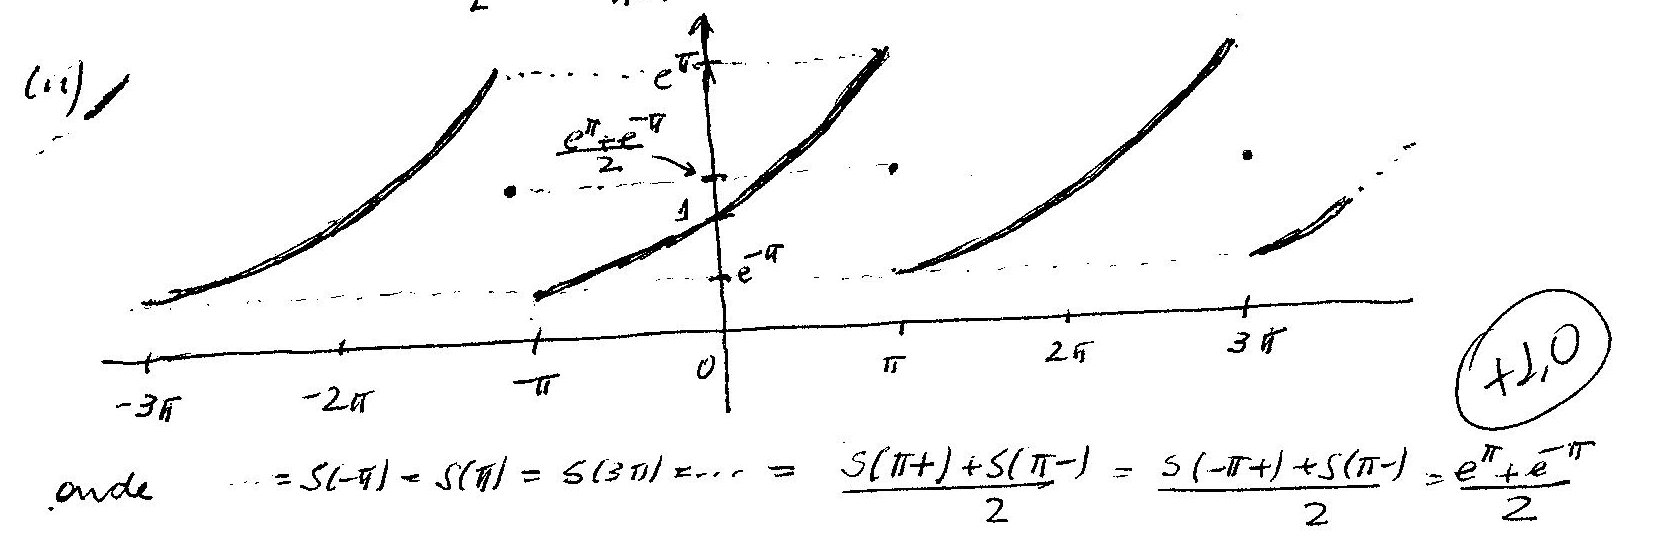
\includegraphics[width=0.8\textwidth]{lista1_fig_p1.jpg}
            \end{center}
        \end{solution}

        \part Use a s\'{e}rie de Fourier para mostrar que
        \begin{align*}
            \sum_{n = 1}^\infty \frac{1}{n^2 + 1} &= \frac{\pi}{2} \coth\left( \pi \right) - \frac{1}{2}.
        \end{align*}
        \begin{solution}
            Tomando $x = \pi$ temos que
            \begin{align*}
                \frac{\exp(\pi) + \exp(-\pi)}{2} &= \cosh\left( \pi \right) \\
                &= \frac{2 \sinh(\pi)}{\pi} \left[ \frac{1}{2} + \sum_{n = 1}^\infty \frac{(-1)^n}{1 + n^2} \left( (-1)^n - n \cdot 0 \right) \right]
            \end{align*}
            e portanto
            \begin{align*}
                \sum_{n = 1}^\infty \frac{1}{1 + n^2} &= \frac{\pi}{2} \coth(\pi) - \frac{1}{2}.
            \end{align*}
        \end{solution}
    \end{parts}

    \question[T1 de 2012] Encontre a s\'{e}rie de Fourier em senos no intervalo $[0,\pi]$ da fun\c{c}\~{a}o $f(x) = x \sin\left( 2 x \right)$, representada abaixo, e fa\c{c}a um gr\'{a}fico da fun\c{c}\~{a}o representada por essa s\'{e}rie para $x \in \mathbb{R}$.
    \begin{center}
        \begin{tikzpicture}[scale=.5]
            \draw[->] (-7,0) -- (7,0) node[below right]{$x$};
            \foreach \x in {1,...,6}{
                \node[below] at (\x,0) {$\x$};
                \node[below] at (-\x,0) {$-\x$};
            }
            \draw[->] (0,-6) -- (0,4.5) node[above right]{$x \sin\left( 2 x \right)$};
            \foreach \x in {1,...,4}{
                \node[left] at (0,\x) {$\x$};
                \node[left] at (0,-\x) {$-\x$};
            }
            \node[left] at (0,-5) {$-5$};
            \node[left] at (0,-6) {$-6$};

            \draw plot[domain=-6.5:6.5, samples=100] (\x, {\x * sin(2 * \x r)});
        \end{tikzpicture}
    \end{center}
    \begin{solution}
        A s\'{e}rie de Foueier em senos \'{e}
        \begin{align*}
            f(x) &= \sum_{n = 1}^\infty b_n \sin\left( n x \right),
        \end{align*}
        onde
        \begin{align*}
            b_n &= \frac{2}{\pi} \int_0^\pi f(x) \sin\left( n x \right) \id{x}.
        \end{align*}

        Portanto,
        \begin{align*}
            b_n &= \frac{2}{\pi} \int_0^\pi x \sin\left( 2 x \right) \sin\left( n x \right) \id{x} \\
            &= \frac{2}{\pi} \int_0^\pi x \frac{1}{2} \left[ \cos\left( 2 x - n x \right) - \cos\left( 2 x + 2 n \right) \right] \id{x} \\
            &= \frac{1}{\pi} \underbrace{\int_0^\pi x \cos\left( \left( n - 2 \right) x \right) \id{x}}_{\bigstar} - \frac{1}{\pi} \underbrace{\int_0^\pi x \cos\left( \left( n + 2 \right) x \right) \id{x}}_{\bigstar\bigstar} \\
            \bigstar &= \begin{cases}
                \left[ (-1)^{n - 2} - 1 \right] \left( n - 2 \right)^{-2}, n \neq 2, \\
                \int_0^\pi x \cos\left( 0 x \right) \id{x} = \pi^2 / 2, n = 2,
            \end{cases} \\
            \bigstar\bigstar &= \underbrace{\left. x \frac{\sin\left( \left( n + 2 \right) x \right)}{n + 2} \right|_0^\pi}_{=0} - \frac{1}{n + 2} \int_0^\pi \sin\left( \left( n + 2 \right) x \right) \id{x} \\
            &= \left. \frac{1}{\left( n + 2 \right)^2} \cos\left( \left( n + 2 \right) x \right) \right|_0^\pi \\
            &= \frac{\left[ \left( -1 \right)^{n + 2} - 1 \right]}{\left( n + 2 \right)^2},
        \end{align*}

        Para $n \neq 2$, temos
        \begin{align*}
            b_n &= \frac{1}{\pi} \left[ \frac{\left[ (-1)^n - 1 \right]}{\left( n - 2 \right)^2} - \frac{\left[ \left( -1 \right)^n - 1 \right]}{\left( n + 2 \right)^2} \right] \\
            &= \frac{1}{\pi} \frac{\left[ \left( -1 \right)^n - 1 \right]}{\left( n^2 - 4 \right)^2} \left[ \left( n + 2 \right)^2 - \left( n - 2 \right)^2 \right] \\
            &= \frac{8 n}{\pi} \frac{\left[ \left( -1 \right)^n - 1 \right]}{\left( n^2 - 4 \right)^2}.
        \end{align*}
        E para $n = 2$, temos
        \begin{align*}
            b_2 &= \frac{1}{\pi} \left[ \frac{\pi^2}{2} - \frac{\left[ \left( -1 \right)^2 - 1 \right]}{\left( 2 + 2 \right)^2} \right] \\
            &= \frac{\pi}{2}.
        \end{align*}

        Por fim,
        \begin{align*}
            f(x) &= \frac{\pi}{2} \sin\left( 2 x \right) + \sum_{n = 1, n \neq 2}^\infty \frac{8 n}{\pi} \frac{\left[ (-1)^n - 1 \right]}{\left( n^2 - 4 \right)^2} \sin\left( n x \right) \\
            &= \frac{\pi}{2} \sin\left( 2 x \right) + \sum_{n = 1, 3, 5, \ldots}^\infty \frac{8 n}{\pi} \frac{\left[ (-1)^n - 1 \right]}{\left( n^2 - 4 \right)^2} \sin\left( n x \right) \\
            &= \frac{\pi}{2} \sin(2 x) - \frac{16}{\pi} \sum_{k = 0}^\infty \frac{\left( 2 k + 1 \right) \sin\left( \left( 2k + 1 \right) x \right)}{\left[ \left( 2 k + 1 \right)^2 - 4 \right]^2}.
        \end{align*}
        \begin{center}
            \begin{tikzpicture}[scale=.8]
                \draw[->] (-7,0) -- (7,0) node[below right]{$x$};
                \foreach \x in {1,...,6}{
                    \node[below] at (\x,0) {$\x$};
                    \node[below] at (-\x,0) {$-\x$};
                }
                \draw[->] (0,-6) -- (0,4.5) node[above right]{$x \sin\left( 2 x \right)$};
                \foreach \x in {1,...,4}{
                    \node[left] at (0,\x) {$\x$};
                    \node[left] at (0,-\x) {$-\x$};
                }
                \node[left] at (0,-5) {$-5$};
                \node[left] at (0,-6) {$-6$};

                \draw plot[domain=0:3.14] (\x, {\x * sin(2 * \x r)});
                \draw[xshift=3.14cm] plot[domain=0:3.14] (\x, {- (3.14 - \x) * sin(2 * (3.14 - \x) r)});
                \draw[xshift=-3.14cm] plot[domain=0:3.14] (\x, {- (3.14 - \x) * sin(2 * (3.14 - \x) r)});
                \draw[xshift=-6.28cm] plot[domain=0:3.14] (\x, {\x * sin(2 * \x r)});
            \end{tikzpicture}
        \end{center}
    \end{solution}
\end{questions}
% \bibliographystyle{plain}
% \bibliography{bibliography}
\end{document}
